\documentclass[11pt]{article}
\usepackage[margin=2.54cm]{geometry}
\usepackage{amsfonts, amsmath, amssymb}
\usepackage{graphicx}
\graphicspath{ {images/} }
\usepackage{hyperref}
\usepackage[shortlabels]{enumitem}
\setlength{\parindent}{0em}

\begin{document}

\thispagestyle{empty}
\tableofcontents
\clearpage
\setcounter{page}{1}

\section{Problem definition} \label{problem_definition}
KPMG's report on "The alcoholic beverages market in Poland" claims, that in 2013, Poles spent 41.1 billion zlotys on alcohol, with beer being a large portion of that amount (47\%) \cite{kpmg_alco}. The report also states that, as of 2014, Polish customers choose beers based on premiumisation (31\% of customers), innovation (29\%) and region affiliations (30\%), with manufacturers predicting significant rise of interest in those attributes in the future \cite{kpmg_alco}. The evolution in customers' taste and their openness resulted in many local shops offering a vast range of, so called, "craft beers" coming from lesser known breweries. However, it's also not uncommon to stumble upon large product shelves, with dozens different beers types, in more popular Polish stores like Lidl and Carrefour.\\

\begin{figure}[h]
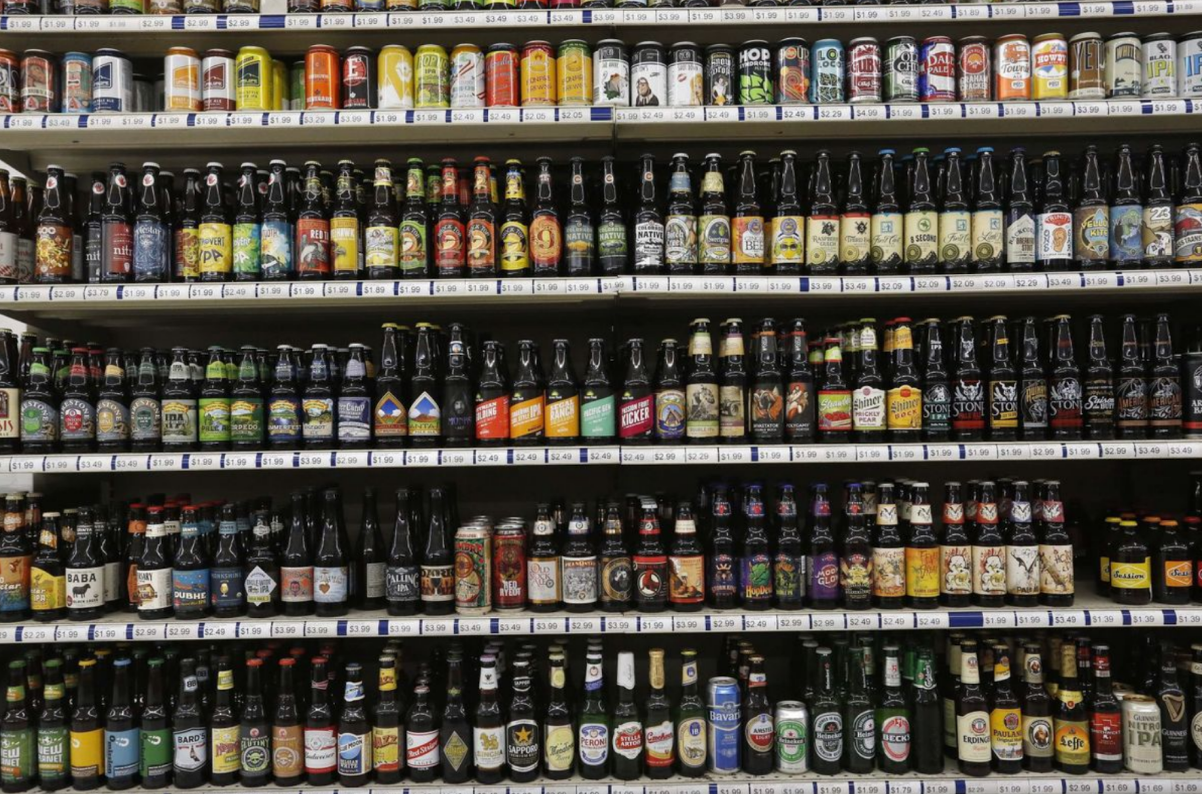
\includegraphics[width=0.5\textwidth]{beer_shelf}
\centering
\caption{A large beer shelf. Source: \protect \url{http://trib.com}.}
\label{fig:beer_shelf}
\end{figure}

The question this thesis posed at first was "How technology could be used to help a customer, who stands in front of a supermarket's large beer shelf (\autoref{fig:beer_shelf}.) and tries to choose one, not knowing anything about beers?". The answer appeared to be relatively simple and involved developing a mobile application, which could connect to beer database residing in Cloud e. g. Firebase Realtime Database and retrieve details about any given beer. The real problem, that later emerged, and is in fact the basis of this thesis, is "Given a mobile application, that can connect to beer database in Cloud, what is the most intuitive, appealing and fastest way of accessing this database from the device?".
\clearpage

\section{Solution overview} \label{solution_overview}
To further investigate the problem articulated in Chapter \ref{problem_definition}, I conducted a survey \cite{survey}. Its main question, that I want to focus on in this section, was "Imagine standing in front of a big shelf with hundreds of craft beers you've never seen before. There's no one there to help you except a mobile app with beer database, which you can access in different ways: typing beer name, using voice to input beer name, making photo of front beer label, making photo of bar code in the back of the bottle. Rank those ways starting from the one that's the most intuitive and appealing to you.". Interestingly, the most popular option, among 50 people asked, was making a photo of front beer label. This method of database access was almost equally popular to the most standard human-device communication interface, which is keyboard (typing a beer name). Whereas \autoref{fig:survey_chart} presents the overall trend, \autoref{fig:survey_table} provides us with detailed numbers: 60\% of people chose, in either first or second place, making a photo of front beer label as their preference (same as in typing a beer name by hand). The last thing that's worth noting is the lack of popularity of barcode scanning.\\

Based on the aforementioned survey and my personal experience, I want to formulate a solution to the problem, stated in Chapter \ref{problem_definition}, as a design and implementation of server-client recognition system for beer labels.

\begin{figure}[h]
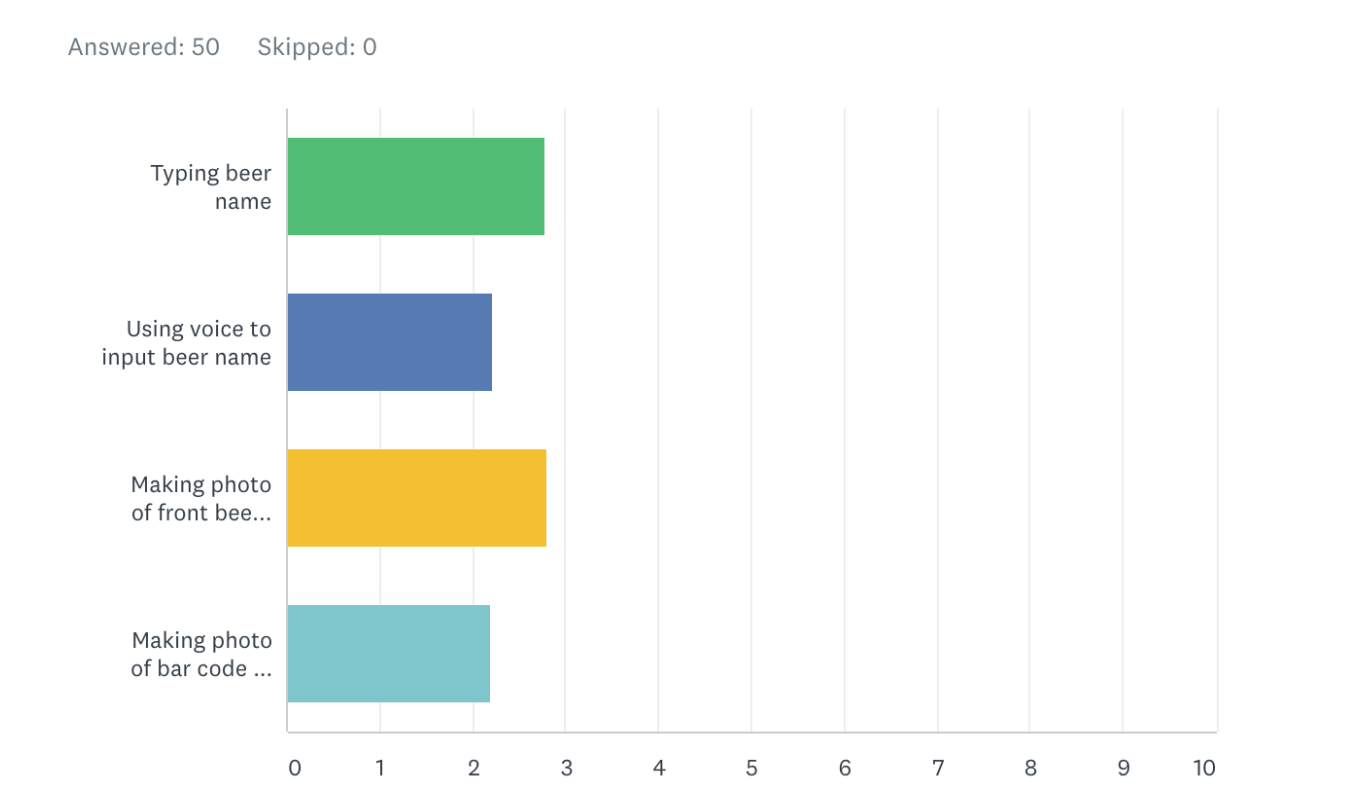
\includegraphics[width=0.5\textwidth]{survey_chart}
\centering
\caption{Weighted average of respondents' answers (chart). For choosing an option as first - weight: 4, for choosing an option as second - weight: 3 etc. Obtained sum is then divided by total number of respondents (here: 50).}
\label{fig:survey_chart}
\end{figure}

\begin{figure}[h]
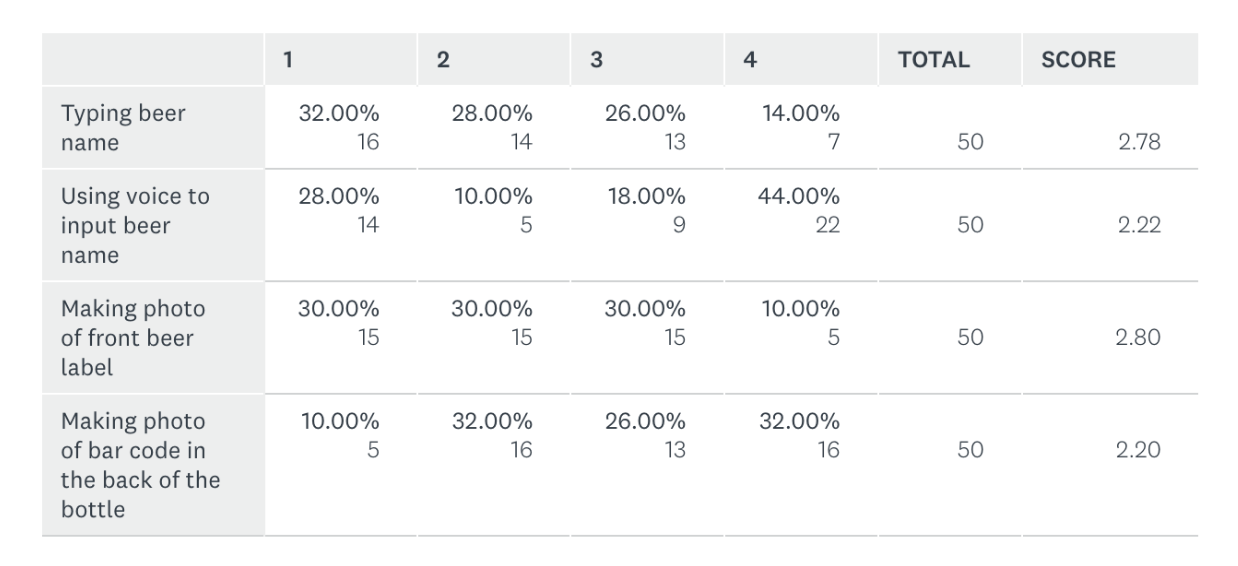
\includegraphics[width=0.5\textwidth]{survey_table}
\centering
\caption{Weighted average of respondents' answers (table with details). For method of average calculation see: \autoref{fig:survey_chart}.}
\label{fig:survey_table}
\end{figure}

The goal of this section is to give a reader, in a few short points, an overall idea of the recognition system before theoretical introduction. Chapter \ref{solution_walkthrough} focuses on implementation details. \autoref{fig:scheme} presents a scheme with a functional principle of implemented server-client beer label recognizer, namely:
\begin{enumerate}
\item An image of beer label is taken by the Android \cite{android_guide} application. 
\item Android application sends the image to the Flask \cite{flask_docs} server equipped with algorithm, which performs beer label prediction.
\item Encoded prediction is returned to Android application.
\item Encoded prediction is used as a key to the beer database residing in Firebase Cloud \cite{firebase_database_docs}.
\item Based on the key (encoded label name) all information about given beer is sent to Android application and displayed to the user.
\end{enumerate}

\begin{figure}[h]
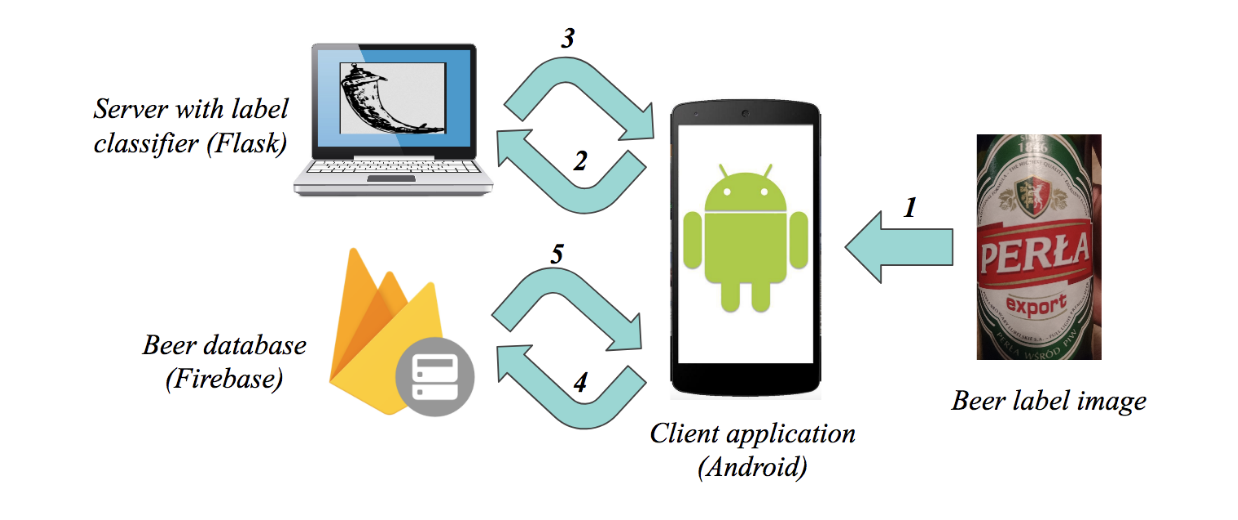
\includegraphics[width=0.5\textwidth]{scheme}
\centering
\caption{Server-client recognition system for beer labels with functional principle (consecutive steps enumerated).}
\label{fig:scheme}
\end{figure}
\clearpage

\section{Introduction to Artificial Intelligence} \label{introduction_to_ai}
There are many approaches to define Artificial Intelligence (AI), but perhaps the most famous is the one formed by Alan Turing in 1950. The proposed method, referred to as Turing test, involved human subject asking written questions to a computer and receiving written answers. If the interrogator couldn't tell if responses came from a human or a machine - the test was passed, i. e. the computer was considered intelligent (at least in some sense). Even stricter rules were imposed on conduction of, so called, total Turing test. In addition to requirements mentioned previously, a computer needed to fool a human subject through a proper visual perception and human-like object manipulations (robotics).\\

Achieving a feat of passing either of aforementioned tests requires multidisciplinary knowledge in many fields. Norvig and Russell did a remarkable job of listing major disciplines, that contributed to the growth of AI \cite{ai_modern_approach}, namely:
\begin{enumerate}[a)]
\item philosophy
\item mathematics
\item economics
\item neuroscience
\item psychology
\item computer engineering
\item control theory and cybernetics
\item linguistics
\end{enumerate}
Despite invaluable contributions from greatest minds in above fields, the Holy Grail of some researchers - Artificial General Intelligence, often called "strong AI", capable of performing any intellectual task of human being - is still far ahead. Focus of many scientists, and also of this thesis, is, conversely, on creating algorithm, which behaves in an intelligent manner in a specific area of expertise (e. g. computer vision), but fails miserably in others (e. g. voice recognition). A big part of this approach revolves around a branch of Artificial Intelligence called supervised learning. \\

In essence, supervised learning is inference of correct outputs from given inputs based on labeled training set. Examples of this include:
\begin{enumerate}[a)]
\item given an email, is it spam or not?
\item given an image, does it contain face or not?
\item given an audio clip, what is the correct transcript?
\item given a Polish sentence, what is semantically correct English translation?
\item given a beer label image, what is the name of the beer?
\end{enumerate}
Prerequisites of performing such tasks are, usually, a large amount of data (e. g. actual emails correctly marked as spam or not) and big computational power (powerful Graphics Processing Units, High-Performance Computing), both of which significantly increased over the past years (\autoref{fig:cpu_gpu}, \autoref{fig:cisco_era}).\\

\begin{figure}[h]
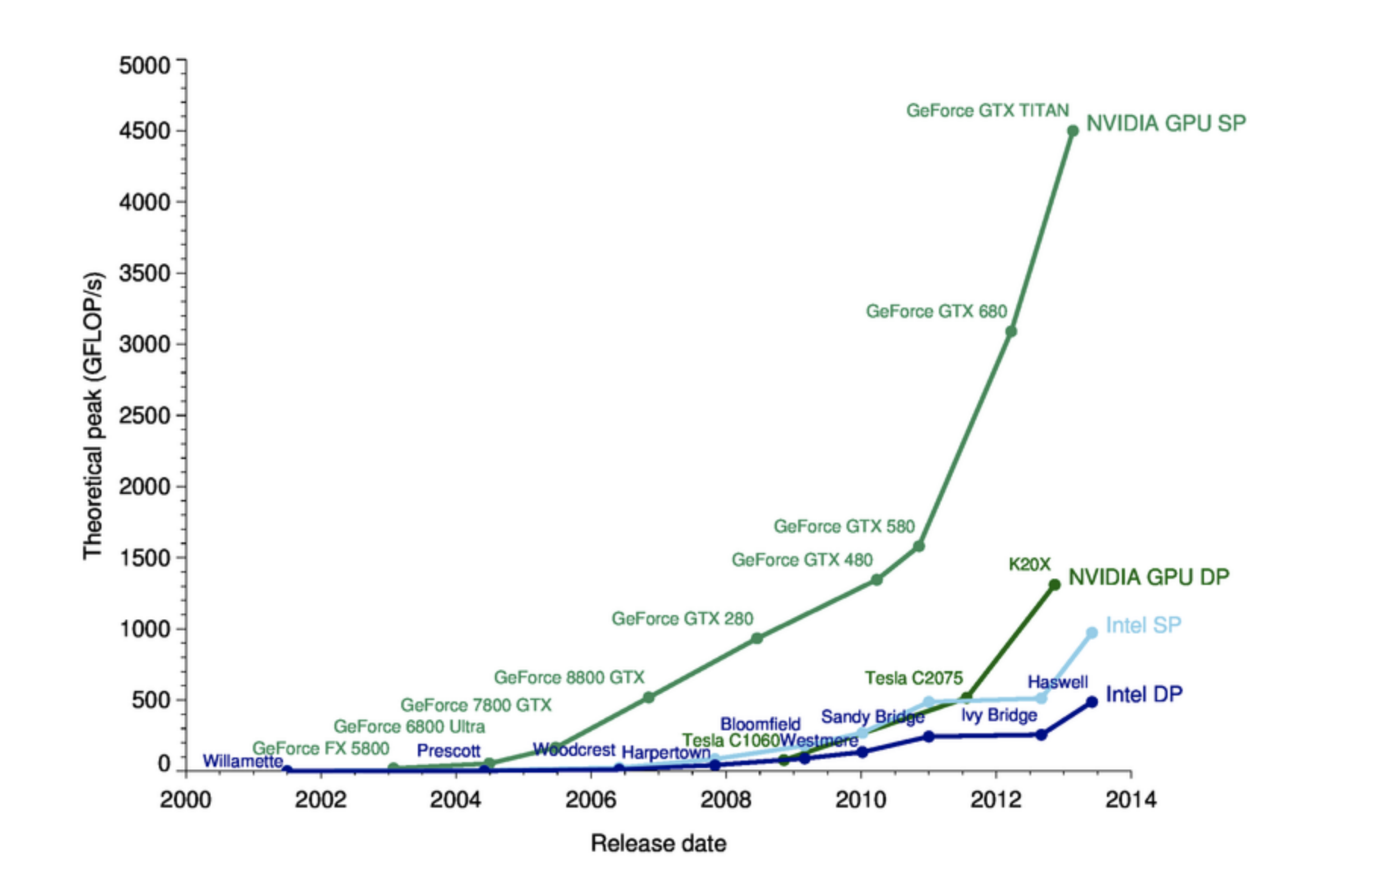
\includegraphics[width=0.5\textwidth]{cpu_gpu}
\centering
\caption{Performance of NVIDIA GPUs and Intel CPUs measured in GFLOP/s \cite{cpu_vs_gpu}.}
\label{fig:cpu_gpu}
\end{figure}

\begin{figure}[h]
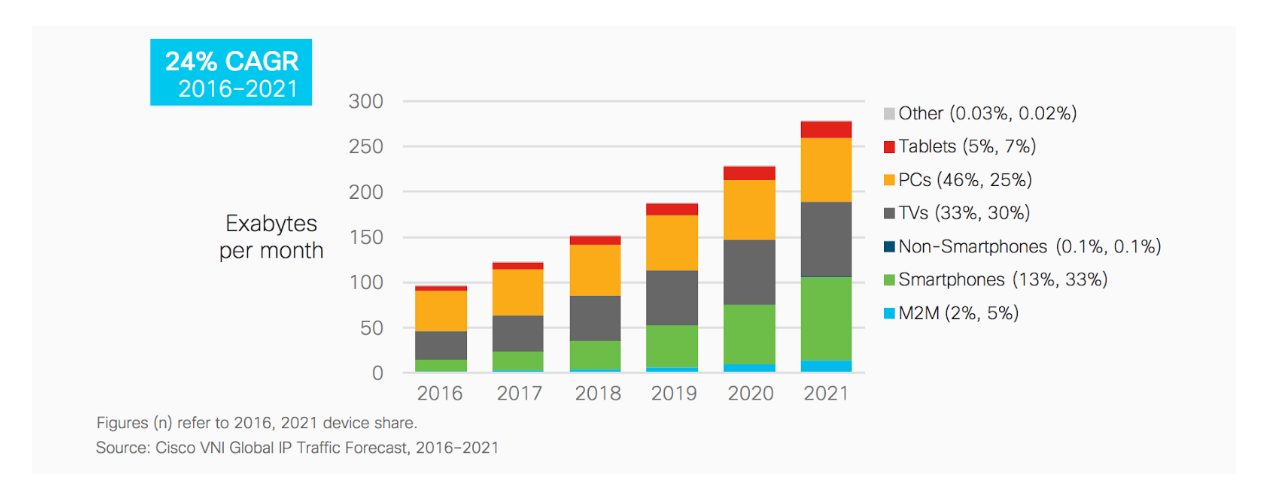
\includegraphics[width=0.5\textwidth]{cisco_era}
\centering
\caption{Global IP traffic by devices \cite{cisco_era} with 24\% compound annual growth rate (2016-2021).}
\label{fig:cisco_era}
\end{figure}

I want to conclude this chapter with important distinction between Machine Learning (ML) and Artificial Intelligence. The former is considered to be a subset of the latter. Whereas AI comprises of knowledge base systems, genetic algorithms, Bayesian statistics etc., none of that is considered ML. Machine Learning can be defined as an act of optimization along a certain dimension (e. g. minimizing the error of choosing a wrong prediction of a beer label based on an image) and a primary tool for that is an algorithm called neural network, loosely based on a human brain cell.
\clearpage

\section{Introduction to Neural Networks} \label{introduction_to_nn}
It's reasonable to think of a neural network (NN) as a mathematical function, which in practice tends to be very complicated because of three things:
\begin{enumerate}[1)]
\item it has a large number of coefficients (weights), often exceeding tens of millions
\item it's a very deeply nested function, hence even simple gradient calculation (partial derivative) is relatively slower
\item most of its computations are performed on multidimensional tensors
\end{enumerate}
\autoref{fig:no_activation_net} contains a popular representation of a simple neural network with three basic building blocks: unit (single circle with value $in_i^{(k)}$, input $x_i$, output $\hat{y_i}$ or bias $1$), layer (units arranged into one vertical group $k$) and weight (connection between units with value $w_{ij}^{(k)}$ representing its strength). Eq. \ref{eq:y_hat_1}, \ref{eq:y_hat_2}, \ref{eq:in_1}, \ref{eq:in_2} and \ref{eq:in_3} translate this graphical representation to mathematical formula.\\

\begin{figure}[h]
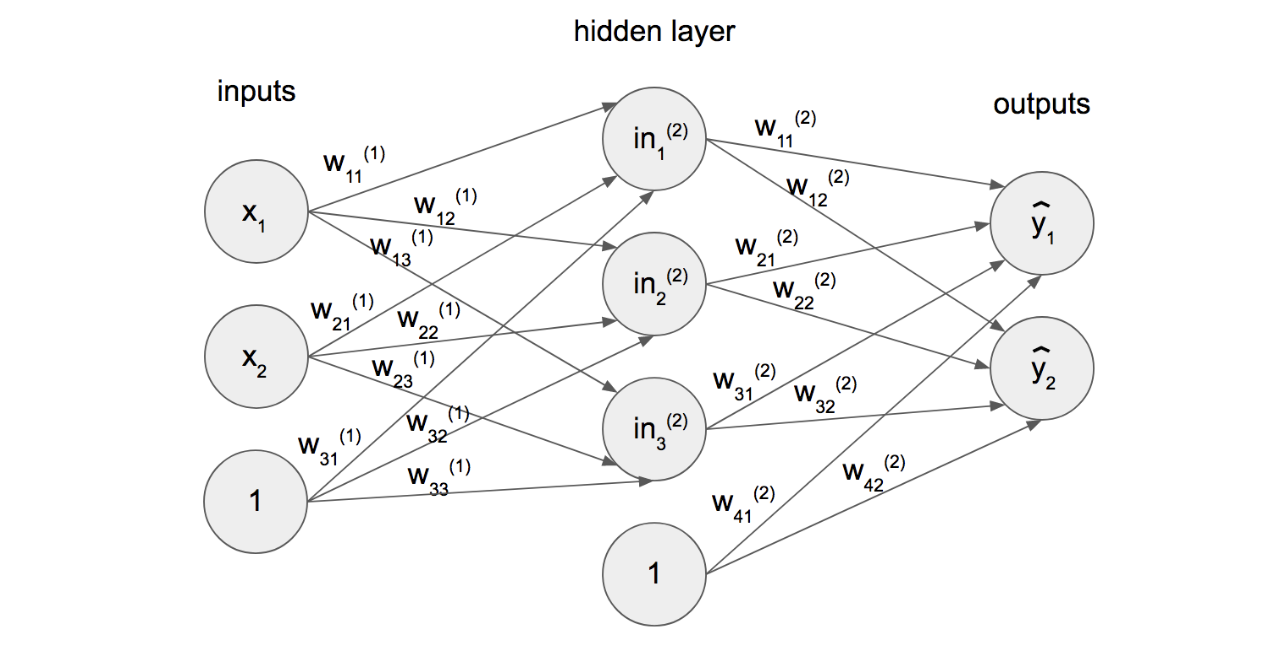
\includegraphics[width=0.5\textwidth]{no_activation_net}
\centering
\caption{A simple neural network with one hidden layer (a layer between inputs and outputs).}
\label{fig:no_activation_net}
\end{figure}

\begin{equation} \label{eq:y_hat_1}
\hat{y_1} = w_{11}^{(2)}in_1^{(2)} + w_{21}^{(2)}in_2^{(2)} + w_{31}^{(2)}in_3^{(2)} + w_{41}^{(2)} * 1 
\end{equation}

\begin{equation} \label{eq:y_hat_2}
\hat{y_2} = w_{12}^{(2)}in_1^{(2)} + w_{22}^{(2)}in_2^{(2)} + w_{32}^{(2)}in_3^{(2)} + w_{42}^{(2)} * 1 
\end{equation}

\begin{equation} \label{eq:in_1}
in_1^{(2)} = w_{11}^{(1)}x_1 + w_{21}^{(1)}x_2 + w_{31}^{(1)} * 1 
\end{equation}

\begin{equation} \label{eq:in_2}
in_2^{(2)} = w_{12}^{(1)}x_1 + w_{22}^{(1)}x_2 + w_{32}^{(1)} * 1 
\end{equation}

\begin{equation} \label{eq:in_3}
in_3^{(2)} = w_{13}^{(1)}x_1 + w_{23}^{(1)}x_2 + w_{33}^{(1)} * 1 
\end{equation}

"Perceptron" is a common name for a neural network, where inputs are immediately coupled with outputs (no hidden layers, unlike in \autoref{fig:no_activation_net}). The presence of hidden (middle) layer of units, which prevents from direct connections between inputs and outputs, allows neural network to model highly nonlinear mathematical functions. Norvig and Russell justify that, using XOR gate as an example, in a following manner: "[...] linear classifiers [...] can represent linear decision boundaries in the input space. This works fine for the carry function, which is a logical AND [...]. The sum function, however, is an XOR (exclusive OR) of the two inputs. [...] this function is not linearly separable so the perceptron cannot learn it. The linearly separable functions constitute just a small fraction of all Boolean functions." \cite{ai_modern_approach}\\

Before delving into learning process of NNs, it's important to make two additions to previous model:
\begin{enumerate}[1)]
\item error function (also called cost function)
\item activation function
\end{enumerate}
Ad 1. The most reliable way for the algorithm to represent predictions is through a vector of probabilities. Consider an example of beer name predictions based on image of label. \autoref{fig:probability_vectors} shows a probability output of a classifier (notice that all values sum to 1), compared with an output, that it should strive for. A cost function I want to introduce in this section, called categorical cross entropy (Eq. \ref{eq:cross_entropy}), simply measures the correlation between those two probability distributions (predicted and ideal). Notice that multiplication by one-hot encoded examples, forces the function to only compare non-zero elements of ideal distribution, with respective values of classifier output further from 1 being penalized more than values close to 1 (thanks to the nature of logarithm).\\ 

\begin{figure}[h]
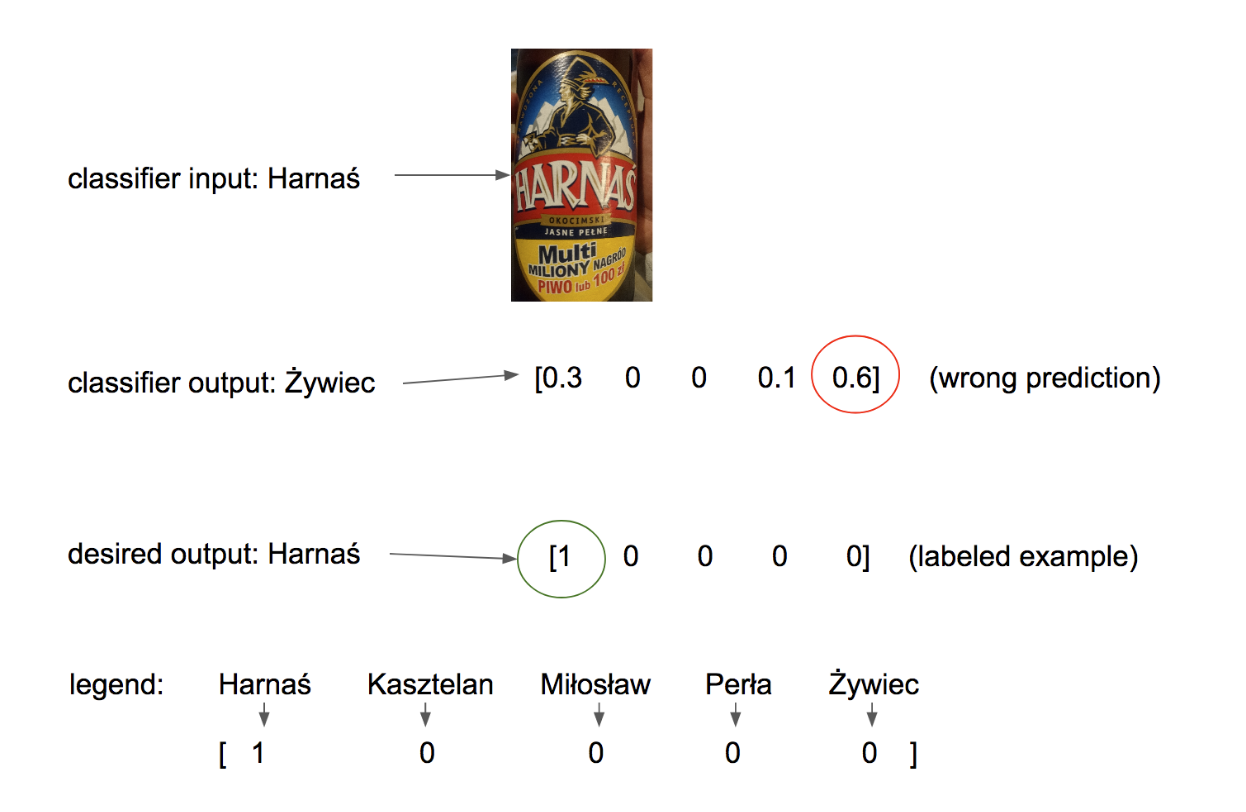
\includegraphics[width=0.5\textwidth]{probability_vectors}
\centering
\caption{Exemplary classifier input, output and desired (one-hot encoded) output with legend.}
\label{fig:probability_vectors}
\end{figure}

\begin{equation} \label{eq:cross_entropy}
H(d, p) = -\sum_i d_i * log(p_i)
\end{equation}
where:
\begin{itemize}
\item[$d_i$] is the $i^{th}$ element of one-hot encoded (desired) probability vector $d$,
\item[$p_i$] is the $i^{th}$ element of probability vector $p$ predicted by the classifier.
\end{itemize}

Ad 2. Unit's value $in_i^{(k)}$ is rarely propagated explicitly to next layers. So called activation function is used instead. The one I'll be introducing in this section is called sigmoid (Eq. \ref{eq:sigmoid}). The updated model of simple neural network from \autoref{fig:no_activation_net} is shown in \autoref{fig:activation_net}. One thing worth pointing out is a difference between sigmoid and softmax function (Eq. \ref{eq:softmax}) - both used in artificial neural networks. Whereas sigmoid inputs a single value and outputs a normalized scalar, softmax inputs a list of values and outputs a vector of real numbers in range [0, 1] that add up to 1, thus can be interpreted as a probability distribution. Sigmoid is used in hidden units, while softmax is usually applied in the last output layer. Both functions can be categorized as logistic functions.\\

\begin{figure}[h]
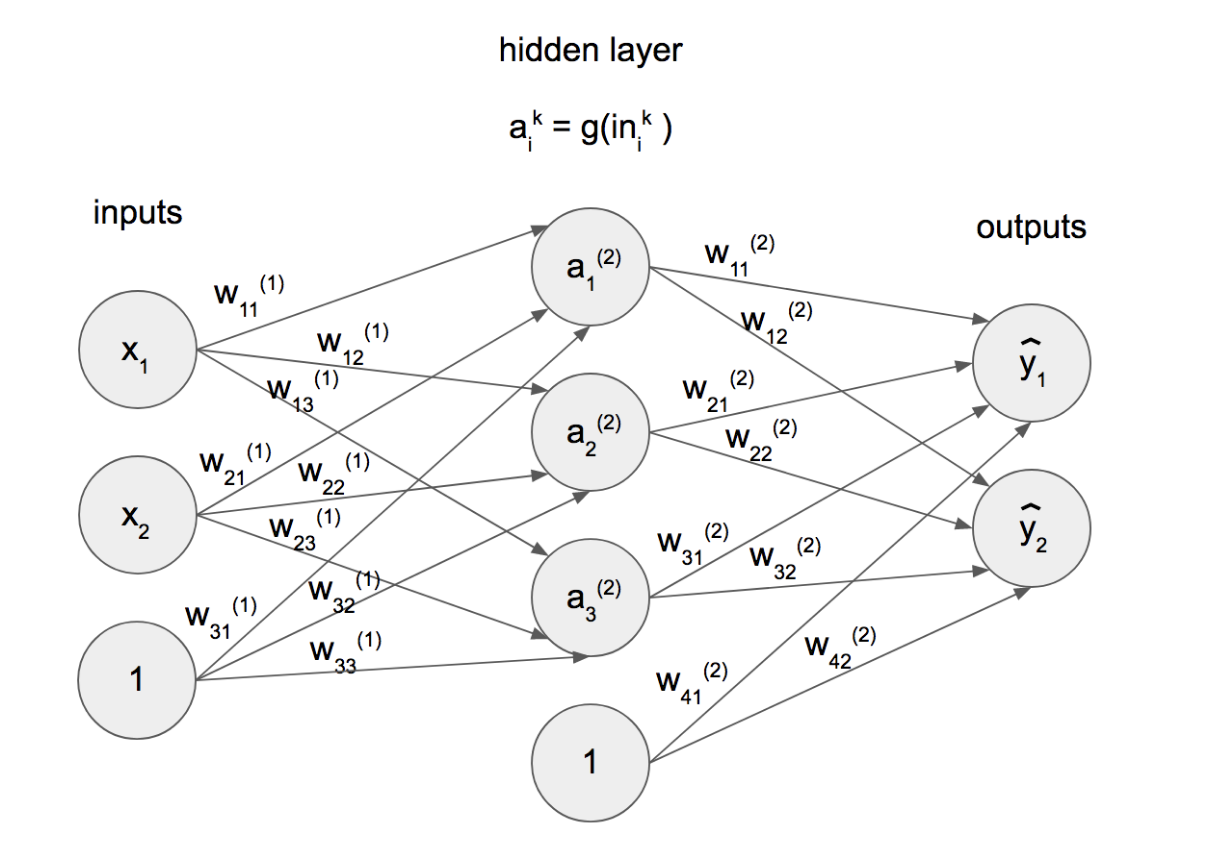
\includegraphics[width=0.5\textwidth]{activation_net}
\centering
\caption{Updated model of simple neural network from \autoref{fig:no_activation_net}. $g$ is a sigmoid activation function. Outputs are often normalized using softmax.}
\label{fig:activation_net}
\end{figure}

\begin{equation} \label{eq:sigmoid}
g(x) = \frac{1}{1 + e^{-x}}
\end{equation}

\begin{equation} \label{eq:softmax}
s(z)_j = \frac{e^{z_j}}{\sum_{k=1}^Ke^{z_k}}
\end{equation}
Softmax function $s(z)_j$ “squashes” a $K$-dimensional vector $z$ to $K$-dimensional probability distribution, where $j=1, ..., K$.\\

The goal of neural network's learning process is to find correct weights, i. e. weights, that will result in a mathematical model, where the difference of inputs is clearly represented in the difference of output vectors, which are subjects to analysis and prediction. For example in a trained dog breed classifier, the output vector for an image of german shepherd is clearly different than for york's. This can be easily interpreted and lead to correct human-readable prediction of a breed. Currently, the best known way to train a network is via algorithm called backpropagation. Main idea of this method is to calculate gradients of a cost function E (e. g. categorical cross entropy) with respect to each of weights, which are later updated by some portion of these gradients as illustrated in Eq. \ref{eq:update_rule}.

\begin{equation} \label{eq:update_rule}
w_{ij}^{'(k)} \leftarrow w_{ij}^{(k)} - \alpha\frac{\partial E}{\partial w_{ij}^{(k)}}
\end{equation}
where:
\begin{itemize}
\item[$\alpha$] is a learning rate (indicating what portion of gradient should be used).
\end{itemize}

Let us consider a neural network in \autoref{fig:simple_net} with three units, one hidden layer and sigmoid activation function. Before conducting backpropagation, I performed, so called, forward pass, which is simply a mathematical inference of outputs, given inputs (Eq. \ref{eq:inference}).\\

\begin{figure}[h]
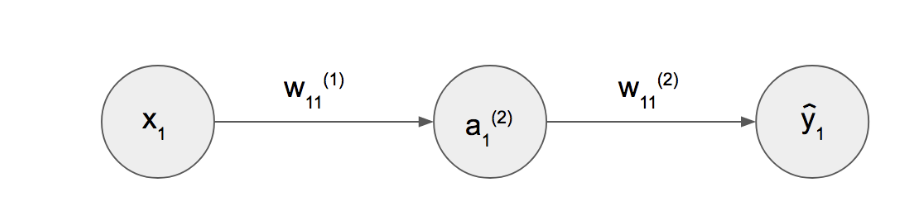
\includegraphics[width=0.5\textwidth]{simple_net}
\centering
\caption{A simple neural network, with sigmoid activation function $g$ (Eq. \ref{eq:sigmoid}), i. e. $a_1^{(2)}=g(w_{11}^{(1)}x_1)$.}
\label{fig:simple_net}
\end{figure}

\begin{equation} \label{eq:inference}
\hat{y_1} = \frac{w_{11}^{(2)}}{1 + e^{-w_{11}^{(1)}x_1}}
\end{equation}

As mentioned previously, NN's learning algorithm is based on calculating partial derivatives with respect to each of weights. A deep nesting of functions, representing more complicated networks, encourages to make use of chain rule \cite{chain_rule_def}. \autoref{fig:backprop} outlines a single step of backpropagation using categorical cross entropy error function $E$. Eq. \ref{eq:gradient_1} and \ref{eq:gradient_2} present symbolic gradient calculations, necessary for learning process to occur. At this point, a beautifully simple derivative of sigmoid function is worth recalling:
\[ s'(x) = \frac{\partial}{\partial x}\frac{1}{1 + e^{-x}}\]
\[s'(x) = \frac{e^{-x}}{(1 + e^{-x})^2} \]
\[s'(x) = \frac{1}{1 + e^{-x}} * \frac{e^{-x}}{1 + e^{-x}}\]
\[ s'(x) = s(x)(1 - s(x))\]

\begin{figure}[h]
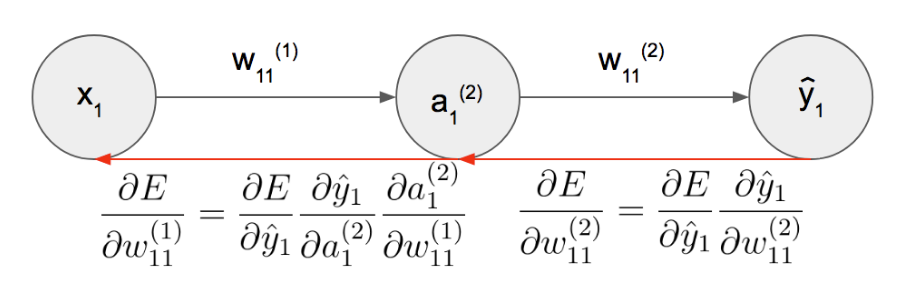
\includegraphics[width=0.5\textwidth]{backprop}
\centering
\caption{Outline of a single step of backpropagation with chain rule, where $E=-y_1log(\hat{y_1})$. Value $y_1$ is a desired binary output from training set.}
\label{fig:backprop}
\end{figure}

\begin{equation} \label{eq:gradient_1}
\frac{\partial E}{\partial w_{11}^{(2)}} = - \frac{y_1}{ln(10) * \hat{y_1}(1 + e^{-w_{11}^{(1)}x_1})}
\end{equation}

\begin{equation} \label{eq:gradient_2}
\frac{\partial E}{\partial w_{11}^{(1)}} = - \frac{w_{11}^{(2)}y_1x_1e^{-w_{11}^{(1)}x_1}}{ln(10) * \hat{y_1}[(1 + e^{-w_{11}^{(1)}x_1})^2]}
\end{equation}

With symbolic computations behind, consider following inputs to neural network from \autoref{fig:backprop}:
\begin{enumerate}[1)]
\item $x_1=10, y_1=1$ - a training example. NN should strive for returning 1, via variable $y_1$, whenever the input is equal to 10.
\item $w_{11}^{(1)}=0.3, w_{11}^{(2)}=0.5$ - randomly initialized weights for first forward pass (Eq. \ref{eq:inference}).
\end{enumerate}
Primary step of learning process is performing inference, given randomly initialized weights and input. The produced outcome is $\hat{y_1} \approx 0.48$, which is quite far from desired 1 ($y_1$). Backward pass allows to calculate gradients with respect to each weight, namely $\frac{\partial E}{\partial w_{11}^{(2)}} \approx 0.86,  \frac{\partial E}{\partial w_{11}^{(1)}} \approx 0.2$. After applying update rule from Eq. \ref{eq:update_rule}, with learning rate $\alpha=0.5$, new weights are $w_{11}^{(1)} \approx 0.4, w_{11}^{(2)} \approx 0.93$ and produce outcome $\hat{y_1} \approx 0.91$(much closer to desired 1). Presented algorithm is iterative. With increased amount of repetitions of above step and larger amount of examples, it should converge to optimal weights (globally or locally).
\clearpage

\section{Introduction to Convolutional Neural Networks} \label{introduction_to_cnns}
\clearpage

\section{Comparison of world-class CNN architectures} \label{comparison_ccn_archs}
\clearpage

\section{Transfer learning} \label{transfer_learning}
\clearpage

\section{Data augmentation} \label{data_augmentation}
\clearpage

\section{Solution walkthrough} \label{solution_walkthrough}
\clearpage

\section{Testing} \label{testing}
\clearpage

\section{Related solutions} \label{related_solutions}
\clearpage

\section{Conclusions} \label{conclusions}
\clearpage

\bibliography{mybib}
\bibliographystyle{siam}

\end{document}